\documentclass[10pt,conference]{IEEEtran}

\ifCLASSINFOpdf
	\usepackage[pdftex]{graphicx}
	%\graphicspath{{./figs/}}
	\DeclareGraphicsExtensions{.pdf,.jpeg,.png}
\else
	\usepackage[dvips]{graphicx}
	%\graphicspath{{./figs/}}
	\DeclareGraphicsExtensions{.eps}
\fi

\usepackage{url}
\usepackage[cmex10]{amsmath}
\usepackage[tight,footnotesize]{subfigure}
\usepackage{xcolor}
\usepackage[lined,ruled]{algorithm2e}
\usepackage{amsmath}

\usepackage[latin1]{inputenc}
\usepackage{tikz}
\usetikzlibrary{shapes}
\usetikzlibrary{arrows}

\usepackage[]{algorithm2e}
\usepackage{graphicx}
\newtheorem{property}{Property}
\newtheorem{proposition}{Proposition}
\newtheorem{theorem}{Theorem}
\newtheorem{conjecture}{Conjecture}
\newtheorem{question}{Question}
\newtheorem{definition}{Definition}
\newtheorem{corollary}{Corollary}

\makeatletter
\pgfdeclareshape{datastore}{
\inheritsavedanchors[from=rectangle]
\inheritanchorborder[from=rectangle]
\inheritanchor[from=rectangle]{center}
\inheritanchor[from=rectangle]{base}
\inheritanchor[from=rectangle]{north}
\inheritanchor[from=rectangle]{north east}
\inheritanchor[from=rectangle]{east}
\inheritanchor[from=rectangle]{south east}
\inheritanchor[from=rectangle]{south}
\inheritanchor[from=rectangle]{south west}
\inheritanchor[from=rectangle]{west}
\inheritanchor[from=rectangle]{north west}
\backgroundpath{
    %  store lower right in xa/ya and upper right in xb/yb
\southwest \pgf@xa=\pgf@x \pgf@ya=\pgf@y
\northeast \pgf@xb=\pgf@x \pgf@yb=\pgf@y
\pgfpathmoveto{\pgfpoint{\pgf@xa}{\pgf@ya}}
\pgfpathlineto{\pgfpoint{\pgf@xb}{\pgf@ya}}
\pgfpathmoveto{\pgfpoint{\pgf@xa}{\pgf@yb}}
\pgfpathlineto{\pgfpoint{\pgf@xb}{\pgf@yb}}
 }
}
\makeatother

\newcommand{\riham}[1]{{\color{red}{#1}}}
\newcommand{\james}[1]{{\color{blue}{#1}}}
\graphicspath{ {images/} }


\begin{document}

\title{Flight Delay Prediction Through Machine Learning}
\author{
\IEEEauthorblockN{Krishna Anantha Padmanabhan}
\IEEEauthorblockA{Rutgers University\\ Piscataway, NJ, USA\\
krishna.ananth@cs.rutgers.edu}
\and
\IEEEauthorblockN{Chintan Trivedi}
\IEEEauthorblockA{Rutgers University\\
 Piscataway, NJ, USA\\
 chintan.trivedi@rutgers.edu}
\and
\IEEEauthorblockN{Raghav Pandya}
\IEEEauthorblockA{Rutgers University\\
Piscataway, NJ, USA\\
raghav.pandya@rutgers.edu}
}

\maketitle
\begin{abstract}
\textnormal{
This project explores the algorithmic approach behind a Prediction System. We study and compare multiple classification algorithms and use the most accurate classifier to predict the possible delay in any flight and Linear Regression to predict the duration of delay. To train this system, we use data collected from the United States Bureau of Transportation Statistics, a data set of various flight journeys.
}
\end{abstract}
%\onecolumn \maketitle \normalsize \vfill

\IEEEpeerreviewmaketitle
%%%%%%%%%%%%%%%%%%%%%%%%%%%%%%%%%%%%%%%%%%%%%%%%%%%%%%%%%%%%%%%%%%%%%%%%%%%%%%%%%%%%%%%%%%%%%%%%%%%%%%%%%
\section{Project Description}\label{sec:1. Project Description}
%%%%%%%%%%%%%%%%%%%%%%%%%%%%%%%%%%%%%%%%%%%%%%%%%%%%%%%%%%%%%%%%%%%%%%%%%%%%%%%%%%%%%%%%%%%%%%%%%%%%%%%%%
\textnormal{
Flight delay predictor system predicts whether the flights will be delayed for departure and then find out the duration of the delay for the flight. For this, we use popular algorithms and techniques from the area of Machine Learning to first learn from the given data and later make predictions from what we have learned. We  train our model for prediction using various attributes of a particular flight such as arrival performance, flight summaries, origin/destination etc. We make use of this model to predict if any future flight will be delayed or not which is to be displayed through a user interface. This system aids flight travelers and air Control staff to get an idea about future flights and if they will be delayed or not. The project is to be completed by three students within a time frame of 6 weeks. The project has four stages: Gathering, Design, Infrastructure Implementation, and User Interface. }

%\subsection{Stage1 - The Requirement Gathering Stage. } \label{sec:1	Requirement Gathering Stage. } 
%\begin{itemize} 
\item{General Description: } 
Our project includes working on the dataset of flights in the USA. We use about 66\% of this data for training multiple classifier algorithms to learn which factors given in our data influence the delay of a flight. We use WEKA data mining tool for this purpose. From that, we classify any flight into two classes, delayed or on-time. We select the classifier model with highest accuracy and use it for amking future predictions. Furthermore, to calculate how much a flight might get delayed, we use a regression model between the attributes of delayed flights as explanatory variables and the time of delay as response variables. The rest of the data is utilized as validation data to analyze the accuracy of this prediction system.    
\item{There are three kinds of users for our prediction system: }

\begin{enumerate}
\item{Flight Traveler: End users who travel through flights.}
\item{Airport Traffic Control staff: Users who have to manage flight schedules and delays.}
\item{Researchers: Users who want to find out what kinds of flights get delayed so they can make scientific improvements.}
\end{enumerate}

\item{The user's interaction modes:
All the users interact with the system through a User Interface developed in Java where they enter flight details to find out if its delayed. We then find if that particular flight belongs to the delayed class of flights or on-time class of flights. For the former case, we then calculate predicted delay in time of the flight.
}

\item{User-wise Scenario: }
\begin{enumerate}
\item{Flight Traveler}
	\begin{itemize}
    \item{Scenario 1 Description: }
    A traveler wants to know if 'AA 2312' on Wednesday, November 1 2015, 9:30 am at Newark(EWR) will arrive late.
    \item{Scenario 1 System Data Input: }
    The flight details are taken as input.
    \item{Scenario 1 Input Data Types: }
    Flight details are airline 'AA' string, flight number '2312' integer, day 'Wednesday' string, date '11/01/2015', time '0930', airport 'EWR' string.
    \item{Scenario 1 System Data Output: }
    Details related to flight arrival delay are given.
    \item{Scenario 1 Output Data Types: }
    Probability of delay of flight and amount of delay in arrival.
    
    \item{Scenario 2 Description: }
    A user wants to arrive at JFK by 10:30 am on Friday, November 13 2015. He has already booked the flight 'DL 666' and wants to know if it'll be delayed so he can catch his connecting flight at 12:00 pm.
    \item{Scenario 2 System Data Input: }
    The flight details are taken as input.
    \item{Scenario 2 Input Data Types: }
	Flight details are airline 'DL' string, flight number '666' integer, day 'Friday' string, date '11/13/2015', time '1030', airport 'JFK' string.
    \item{Scenario 2 System Data Output: }
    Details related to flight arrival delay are given.
    \item{Scenario 1 Output Data Types: }
    Probability of delay of flight and amount of delay in arrival.
    


	\end{itemize}

\item{Air Traffic control staff}
    \begin{itemize} 
    
   	\item{Scenario 1 Description: }
    Air traffic controller wants to know arrival status of flight 'AI 202' arriving at 'Heathrow Airport' on date '12/11/2015' to alocate it an airstrip to land
	\item{Scenario 1 System Data Input:}
	Flight details are airline 'AI' string, flight number '202' integer, day 'Friday' string, date '11/13/2015', time '1030', airport 'LHR' string.
	\item{Scenario 1 System Data Output: }
    Delay in hours and minutes for the given flight
   	\item{Scenario 2 Description: }
    Air traffic controller wants to know arrival status of flight 'KU 303' arriving at 'Newark Liberty Airport' on '10/13/2015' to assign a conveyer belt for luggages for the arrival time
	\item{Scenario 2 System Data Input: }
    Flight details are airline 'KU' string, flight number '303' integer, date '11/13/2015', airport 'EWR' string.
	\item{Scenario 2 System Data Output: }
    Delay in hours and minutes for the given flight

    \end{itemize}

    

    \item{Researchers:}
\begin{itemize} 

	\item{Scenario 1 Description: }
    The researcher wants to know what percentage of flights of the airlines 'AA' are delayed.
	\item{Scenario 1 System Data Input: }
 The name of the airlines.    
    \item{Scenario 1 Input Data Types: }
    Airline name as 'AA' string.
    \item{Scenario 1 System Data Output: }
    The percentage of flights of the airline 'AA' that have faced delay issues.
    \item{Scenario 1 Output Data Types: }
    Percentage value in double of delay of flights of the airline 'AA'.
    
    \item{Scenario 2 Description: }
    Researcher wants to know how many flights are delayed for any given airport, say 'JFK'.
    \item{Scenario 2 System Data Input: }
    The airport name is taken as input.
    \item{Scenario 2 Input Data Types: }
	Airport name 'JFK' in string format.
    \item{Scenario 2 System Data Output: }
    The percentage of flights on the airport 'JFK' that have faced delay issues.
    \item{Scenario 1 Output Data Types: }
    Percentage value in double of delay of flights on the airport 'JFK'.
    
    \end{itemize}
\end{enumerate}    

\item{Project Time line and Division of Labor.}
There are three main components in the project:
\begin{itemize} 

\item{Development of Naive Bayes Tree Classifier on WEKA}
\item{Training the classifier with the dataset and creation of a prediction model with linear regression that will be used while creating a user interface in JAVA}
\item{Testing the implementation with different user levels to establish its stability and maintainability}
\end{itemize}

Each team member will be responsible for one of the components but will be assisted by other team members when needed. Each member will therefore be responsible for design, development, testing and documentation respectively. Krishna would work on generating classifier models and comparing them and store the best classifier model on the disk. Chintan would work on creating the Regression model and storing it on disk and the user interface. Raghav would work on data curation, implementation, analysis and testing at different user levels. The estimated time to complete the project would be around 6 weeks.

\begin{itemize} 
	\item{Week 1: We expect to curate the dataset by the end of the first week. At this stage we will work on identifying the necessary and relevant features that will be required for our application since the BTS dataset contains a lot of irrelevant data. This data curation will be done using python scripts.}
    \item{Week 2: After the dataset is curated, we expect to complete the development of Naive Bayes Tree classifier as a plugin for WEKA by the end of week 2.}
    \item{Week 3: We expect to train the classifiers with our dataset and develop the linear regression prediction model for it. At the same time we will develop a user interface in JAVA for our model.}
    \item{Week 4: We would look at how different user levels can work seamlessly with the application. Its tractability will be the main concern at this stage.}
    \item{Week 5: In this week, testing will be done and we will make the application stable.}
    \item{Week 6: Once the application is stable and maintainable, we expect to complete the project with relevant results and work on the documentation, such as project report and presentation.}
    \end{itemize}
\end{itemize}
\subsection{Stage1 - The Requirement Gathering Stage. }\label{sec:1 Requirement Gathering Stage. }
%%%%%%%
\begin{itemize} 
\item{General Description: } 
Our project includes working on the dataset of flights in the USA. We use about 66\% of this data for training multiple classifier algorithms to learn which factors given in our data influence the delay of a flight. We use WEKA data mining tool for this purpose. From that, we classify any flight into two classes, delayed or on-time. We select the classifier model with highest accuracy and use it for amking future predictions. Furthermore, to calculate how much a flight might get delayed, we use a regression model between the attributes of delayed flights as explanatory variables and the time of delay as response variables. The rest of the data is utilized as validation data to analyze the accuracy of this prediction system.    
\item{There are three kinds of users for our prediction system: }

\begin{enumerate}
\item{Flight Traveler: End users who travel through flights.}
\item{Airport Traffic Control staff: Users who have to manage flight schedules and delays.}
\item{Researchers: Users who want to find out what kinds of flights get delayed so they can make scientific improvements.}
\end{enumerate}

\item{The user's interaction modes:
All the users interact with the system through a User Interface developed in Java where they enter flight details to find out if its delayed. We then find if that particular flight belongs to the delayed class of flights or on-time class of flights. For the former case, we then calculate predicted delay in time of the flight.
}

\item{User-wise Scenario: }
\begin{enumerate}
\item{Flight Traveler}
	\begin{itemize}
    \item{Scenario 1 Description: }
    A traveler wants to know if 'AA 2312' on Wednesday, November 1 2015, 9:30 am at Newark(EWR) will arrive late.
    \item{Scenario 1 System Data Input: }
    The flight details are taken as input.
    \item{Scenario 1 Input Data Types: }
    Flight details are airline 'AA' string, flight number '2312' integer, day 'Wednesday' string, date '11/01/2015', time '0930', airport 'EWR' string.
    \item{Scenario 1 System Data Output: }
    Details related to flight arrival delay are given.
    \item{Scenario 1 Output Data Types: }
    Probability of delay of flight and amount of delay in arrival.
    
    \item{Scenario 2 Description: }
    A user wants to arrive at JFK by 10:30 am on Friday, November 13 2015. He has already booked the flight 'DL 666' and wants to know if it'll be delayed so he can catch his connecting flight at 12:00 pm.
    \item{Scenario 2 System Data Input: }
    The flight details are taken as input.
    \item{Scenario 2 Input Data Types: }
	Flight details are airline 'DL' string, flight number '666' integer, day 'Friday' string, date '11/13/2015', time '1030', airport 'JFK' string.
    \item{Scenario 2 System Data Output: }
    Details related to flight arrival delay are given.
    \item{Scenario 1 Output Data Types: }
    Probability of delay of flight and amount of delay in arrival.
    


	\end{itemize}

\item{Air Traffic control staff}
    \begin{itemize} 
    
   	\item{Scenario 1 Description: }
    Air traffic controller wants to know arrival status of flight 'AI 202' arriving at 'Heathrow Airport' on date '12/11/2015' to alocate it an airstrip to land
	\item{Scenario 1 System Data Input:}
	Flight details are airline 'AI' string, flight number '202' integer, day 'Friday' string, date '11/13/2015', time '1030', airport 'LHR' string.
	\item{Scenario 1 System Data Output: }
    Delay in hours and minutes for the given flight
   	\item{Scenario 2 Description: }
    Air traffic controller wants to know arrival status of flight 'KU 303' arriving at 'Newark Liberty Airport' on '10/13/2015' to assign a conveyer belt for luggages for the arrival time
	\item{Scenario 2 System Data Input: }
    Flight details are airline 'KU' string, flight number '303' integer, date '11/13/2015', airport 'EWR' string.
	\item{Scenario 2 System Data Output: }
    Delay in hours and minutes for the given flight

    \end{itemize}

    

    \item{Researchers:}
\begin{itemize} 

	\item{Scenario 1 Description: }
    The researcher wants to know what percentage of flights of the airlines 'AA' are delayed.
	\item{Scenario 1 System Data Input: }
 The name of the airlines.    
    \item{Scenario 1 Input Data Types: }
    Airline name as 'AA' string.
    \item{Scenario 1 System Data Output: }
    The percentage of flights of the airline 'AA' that have faced delay issues.
    \item{Scenario 1 Output Data Types: }
    Percentage value in double of delay of flights of the airline 'AA'.
    
    \item{Scenario 2 Description: }
    Researcher wants to know how many flights are delayed for any given airport, say 'JFK'.
    \item{Scenario 2 System Data Input: }
    The airport name is taken as input.
    \item{Scenario 2 Input Data Types: }
	Airport name 'JFK' in string format.
    \item{Scenario 2 System Data Output: }
    The percentage of flights on the airport 'JFK' that have faced delay issues.
    \item{Scenario 1 Output Data Types: }
    Percentage value in double of delay of flights on the airport 'JFK'.
    
    \end{itemize}
\end{enumerate}    

\item{Project Time line and Division of Labor.}
There are three main components in the project:
\begin{itemize} 

\item{Development of Naive Bayes Tree Classifier on WEKA}
\item{Training the classifier with the dataset and creation of a prediction model with linear regression that will be used while creating a user interface in JAVA}
\item{Testing the implementation with different user levels to establish its stability and maintainability}
\end{itemize}

Each team member will be responsible for one of the components but will be assisted by other team members when needed. Each member will therefore be responsible for design, development, testing and documentation respectively. Krishna would work on generating classifier models and comparing them and store the best classifier model on the disk. Chintan would work on creating the Regression model and storing it on disk and the user interface. Raghav would work on data curation, implementation, analysis and testing at different user levels. The estimated time to complete the project would be around 6 weeks.

\begin{itemize} 
	\item{Week 1: We expect to curate the dataset by the end of the first week. At this stage we will work on identifying the necessary and relevant features that will be required for our application since the BTS dataset contains a lot of irrelevant data. This data curation will be done using python scripts.}
    \item{Week 2: After the dataset is curated, we expect to complete the development of Naive Bayes Tree classifier as a plugin for WEKA by the end of week 2.}
    \item{Week 3: We expect to train the classifiers with our dataset and develop the linear regression prediction model for it. At the same time we will develop a user interface in JAVA for our model.}
    \item{Week 4: We would look at how different user levels can work seamlessly with the application. Its tractability will be the main concern at this stage.}
    \item{Week 5: In this week, testing will be done and we will make the application stable.}
    \item{Week 6: Once the application is stable and maintainable, we expect to complete the project with relevant results and work on the documentation, such as project report and presentation.}
    \end{itemize}
\end{itemize}

\subsection{Stage2 - The Design Stage. }\label{sec: 2:The Design Stage.}
%%%%%%%%%%%%%%%%%%%%%%%%%%%%%%%%%%%%%%%%%%%%%%%%%%%%%%%%%%%%%%%%%%%%%%%%%%%%%%%%%%%%%%%%%%%%%%%%%%%%%%%%%%
\textnormal{
In this stage, we specify the flow of our system by showing steps in data curation, how we plan to implement classifiers and use its model for prediction as well as the Regression model and connect this with the classifier model. Then, we show how each model is generated by looking at the high level pseudo code for the classifier and the regressor and detail how it is to be implemented. We also specify the data structures that are to be used and take a look at the expected time and space complexity for the same.\\ }
\begin{itemize} 
\item{  System Flow Description. }
The system utilizes the flights training data to develop the models. At the first step, the classifiers takes the flights data as input and create a model that is stored in the disk. This model is then used for predicting if any given flight is to be classified as on-time or delayed. For all the flights classified as delayed, we develop a regression model at the next step and store this model in the disk. This model will help us to estimate by how much time any given flight is delayed. The following two flowcharts explores the system flow chart at high level between the two major components of this system, classifier and regressor. The Fig. 1 flowchart details about generating the classification model and then based on its model conditions when we implement the regressor. The Fig. 2 flowchart details what the flow is when any user enters any input to the system. Here, the models stored in the disk during the earlier stage are utilized for prediction.  
\begin{figure}
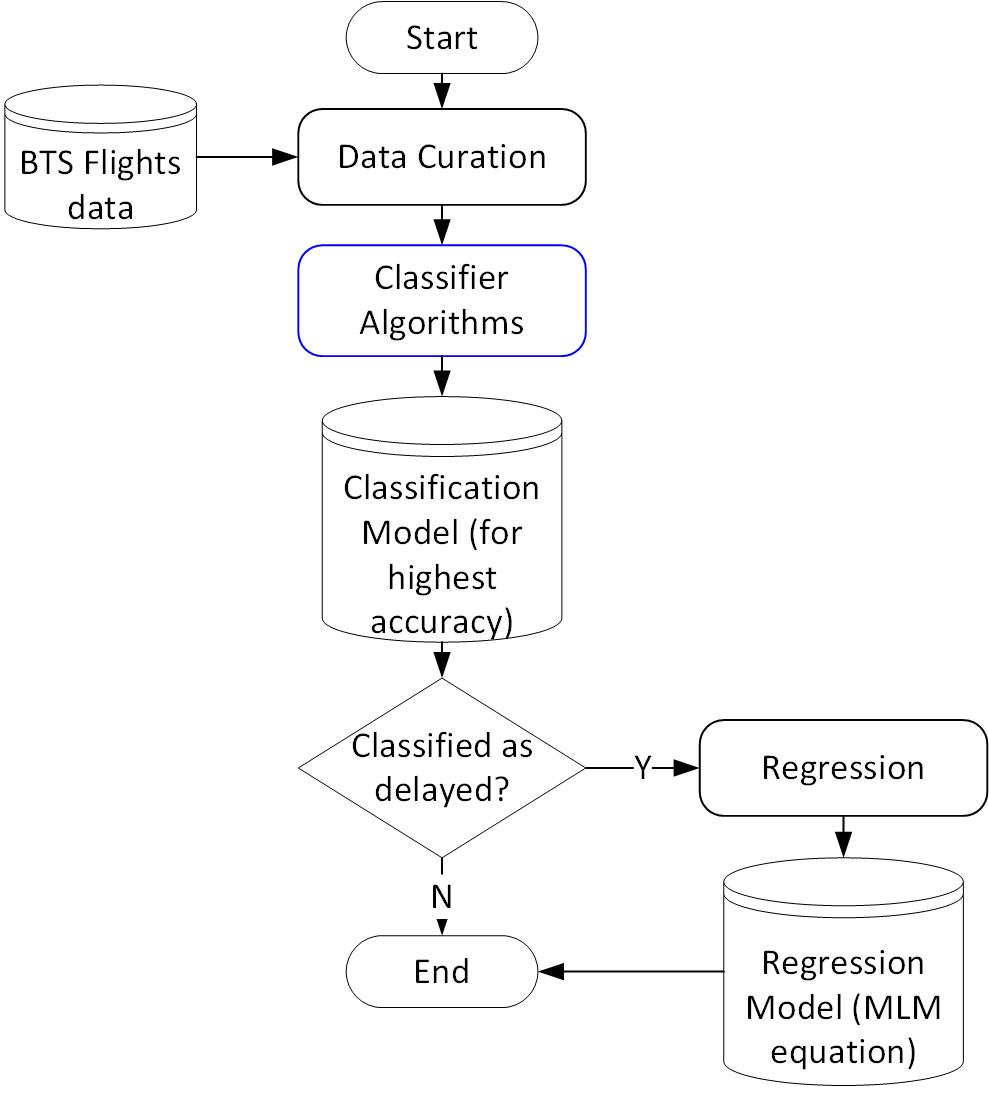
\includegraphics[height=230pt,width=\linewidth]{ModelGen.jpg}
\caption{Flow Diagram for generating Classification and Regression Models.}
\end{figure}
\begin{figure}
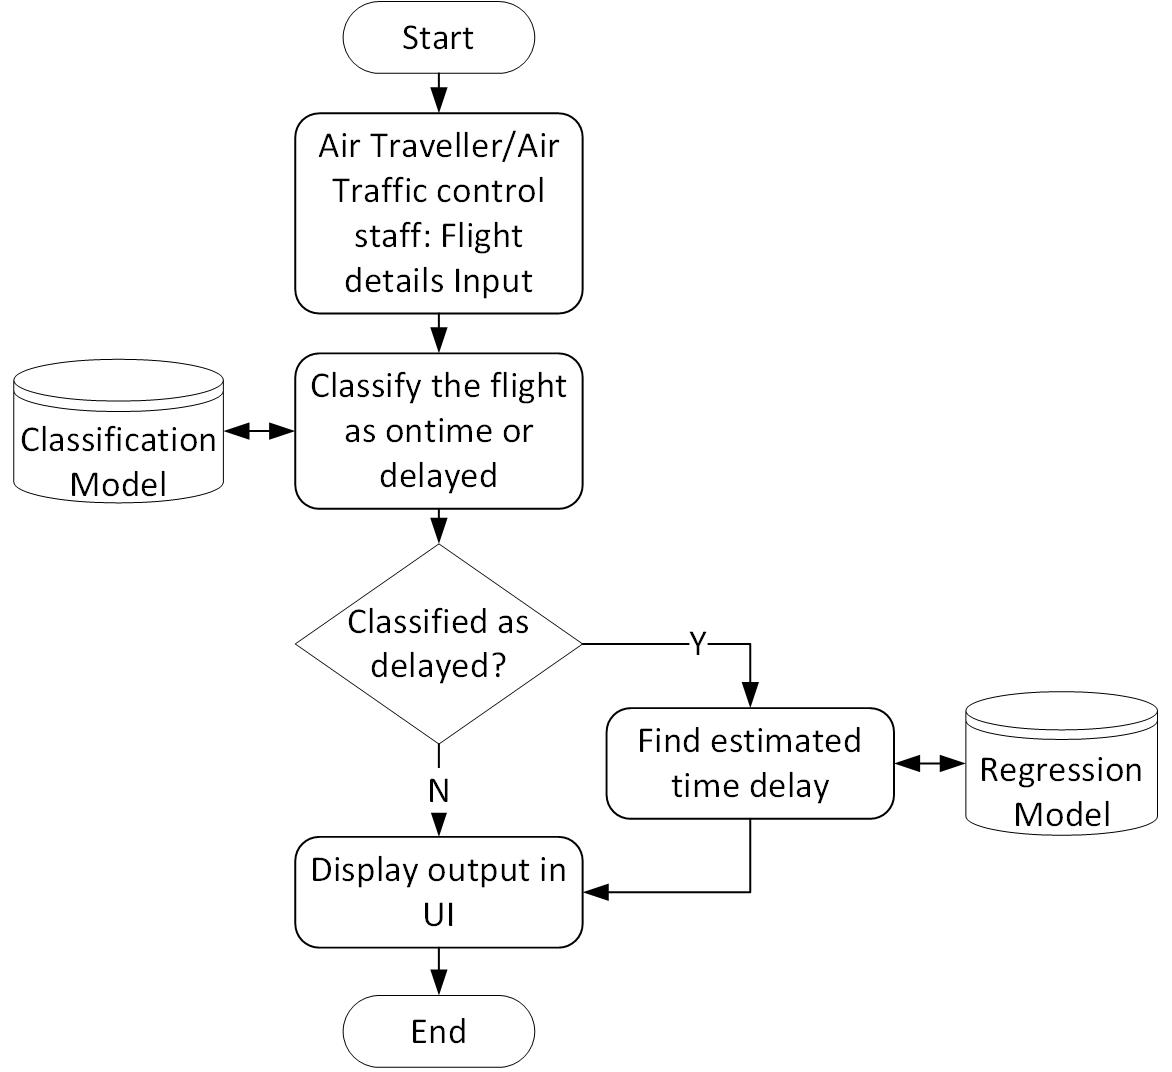
\includegraphics[width=\linewidth]{UserIP.jpg}
\caption{Flow Diagram for making predictions after taking the user input.}
\end{figure}
\\
\\
\\
\item{ High Level Pseudo Code of the system. }
$\\Begin:$

\begin{enumerate}
\item{$data\ =\ read(BTS\_flight\_data)$}
\item{$data \gets Data\_Curation(data)$}
\item{$classes\ =\ \{on\ time,\ delayed\}$}
\item{$Classification(data,classes)$}
\item{$data\_delayed \gets data\ classified\ as\ delayed$}
\item{$Linear\_Regression(data\_delayed)$}
\end{enumerate}
$End\\\\$
\item{Major Algorithms/Components in the Pseudo-code: }
\begin{enumerate}
\item{Data Curation: }
In this algorithmic component, we make sure that the data given as input to the classifier is curated. This is to try and make the classifier as accurate as possible. Following steps detail what actions we plan to take to curate the data.
\begin{itemize}
\item{ Remove records from csv file for which a field is empty (Incomplete records)}
\item{ Create 2 copies of dataset 
\\	1. Numeric : Preserves numeric values 
\\	2. Discretized : Maps Distance, Departure, Arrival time into intervals
\\\textit{Distance}: 
\\Assign interval id from 1 to 11 based on the distance covered(1: 0 to 250 miles, 2: 250 to 500 miles......11: 2500 to 2750 miles)
\\\textit{DEPARTURE TIME, ARRIVAL TIME}: 
\\Assign interval id from 1 to 3 based on the time of day(1: 12am to 8pm, 2: 8pm to 4pm, 3: 4pm to 12am)
}
\item{Randomize the records using WEKA}
\item{Remove flights with uncommon attribute values in ORIGIN/DESTINATION by choosing the Top 25 frequently occurring airports and discarding records for other airports}
\item{Remove flights with uncommon attribute values in CARRIER by choosing only Top 8 commercial airlines and discarding records for other airlines}
\item{Resample the data using WEKA}
\item{Divide the dataset into TRAINING and TESTING dataset in 3:1 ratio}
\end{itemize}

\item{Classifier: We use two main types of classifiers, namely Naive Bayes Tree and J48 Decision Trees. Apart from these, we also use Random Forest, Rule-based classifier and Simple Naive Bayes classifier for comparisons.}
\begin{itemize}
\item{Naive Bayes Tree Algorithm: This algorithm is similar to the classical recursive partitioning schemes, except that the leaf nodes created are Naive-Bayes categorizers instead of nodes predicting a single class. A threshold is chosen using decision trees and the utility of a node is computed by discretizing the data and computing the 5-fold cross-validation accuracy estimate of using Naive-Bayes at the node. The utility of a split is the weighted sum of the utility of the nodes, where the weight given to a node is proportional to the number of instances that go down to that node. The algorithm is as follows:}
\vspace{2.5 mm}
\\*Input: a set $T$ of labeled instances.
\\*Output: a decision tree with Naive-Bayes categorizers at the leaves.
\vspace{0.1 mm}
\begin{itemize}
\item{For each attribute $X_{i}$ evaluate the utility, $u(X_{i})$ of a split on attribute $X_{i}$. For continuous attributes, a threshold is also found at this stage.}
\item{Let $j = $ arg max$_{i}$$(u_{i})$, $i.e.$, the attribute with the highest utility.}
\item{If $u_{j}$ is not significantly better than the utility of the current node, create a Naive-Bayes classifier for the current node and return.}
\item{Partition $T$ according to the test on $X_{j}$. If $X_{j}$ is continuous, a threshold split is used; if $X_{j}$ is discrete, a multi-way split is made for all possible values.}
\item{For each child, call the algorithm recursively on the portion of $T$ that matches the test leading to the child.}
\end{itemize}

If there are $m$ instances, $n$ attributes and $l$ label values, the complexity of the attribute selection phase for discretized attributes is $O(m.n^{2}.l)$. In our case, the number of attributes is less than $O$(log$m$) and the number of labels is small. Hence the time spent on attribute selection using cross-validation is less than the time spent sorting the instances by each attribute. Thus NBTree scales up well to our large database.
\vspace{2.5 mm}
\item{J48 Decision Trees: J48 is an open source implementation of the C4.5 machine learning algorithm which creates decision trees based on the ID3 algorithm, using information entropy and information gain. Entropy is a measure of unpredictability of information content and expected information gain is the change in information entropy $H$ from a prior state to a state that takes some information as given: $IG(T,a) = H(T) - H(T|a)$. This algorithm has a few base cases:
\begin{itemize}
\item{All the samples in the list belong to the same class. When this happens, it simply creates a leaf node for the decision tree saying to choose that class.}
\item{None of the features provide any information gain. In this case, C4.5 creates a decision node higher up the tree using the expected value of the class.}
\item{Instance of previously-unseen class encountered. Again, C4.5 creates a decision node higher up the tree using the expected value.}
\end{itemize} 
The C4.5 or J48 algorithm is as follows:}
\vspace{2.5 mm}
\\*Input: Training data set $S = {s_1, s_2, ...}$ of already classified samples. Each sample  $s_i$ consists of a p-dimensional vector $(x_{1,i}, x_{2,i}, ...,x_{p,i})$ , where the  $x_j$  represent attribute values or features of the sample, as well as the class in which  $s_i$  falls.
\\*Output: Decision tree
\vspace{0.1 mm}
\begin{itemize}
\item{Check for base cases}
\item{For each attribute $a$ Find the normalized information gain ratio from splitting on $a$}
\item{Let $a_{best}$ be the attribute with the highest normalized information gain}
\item{Create a decision node that splits on $a_{best}$}
\item{Recur on the sublists obtained by splitting on $a_{best}$, and add those nodes as children of node}
\end{itemize}

\item{Random Forest: Random forests is a notion of the general technique of random decision forests that are an ensemble learning method for classification, regression and other tasks, that operate by constructing a multitude of decision trees at training time and outputting the class that is the mode of the classes (classification) or mean prediction (regression) of the individual trees. Random decision forests correct for decision trees' habit of overfitting to their training set.}

\item{Rule-based classifier: Rule-based classifier makes use of a set of $IF-THEN$ rules for classification. One rule is created for each path from the root to the leaf node. To form a rule antecedent(the $IF$ part), each splitting criterion is logically $ANDed$. The leaf node holds the class prediction, forming the rule consequent(the $THEN$ part). Such rules are then extracted using a sequential covering algorithm and then pruned due to the following reasons: }
\begin{itemize}
\item{Assessment of quality is made on the original set of training data. The rule may perform well on training data but less well on subsequent data. Hence rule pruning is required.}
\item{The rule is pruned by removing conjunct. A rule R is pruned, if pruned version of R has greater quality than what was assessed on an independent set of tuples.}
\end{itemize}

\item{Simple Naive Bayes classifier: Naive Bayes classifier is a simple probabilistic classifier which is based on Bayes theorem with strong and naive independence assumptions. In other words, Bayes' theorem is used in the classifier's decision rule.  Despite the naive design and oversimplified assumptions that this technique uses, Naive Bayes performs well in many complex real-world problems.
Even though it is often outperformed by other techniques such as boosted trees, random forests, Max Entropy, Support Vector Machines etc, Naive Bayes classifier is very efficient since it is less computationally intensive (in both CPU and memory) and it requires a small amount of training data. Moreover, the training time with Naive Bayes is significantly smaller as opposed to alternative methods.
Its performance is very close to more complicated and slower techniques in many cases.}
\end{itemize}

\item{Linear Regression:}
In this component, we obtain the multiple linear regression model as a linear relationship between the delay in time acting as our response variable and the attributes of the flight like departure airline, airport, departure time, etc. acting as our explanatory variables. For our regressor, we represent these attributes as a matrix of features $(X_{n\times m})$ for all flights. $X_{ij}$ denotes the $j^{th}$ feature of the $i^{th}$ flight record.
\[
X_{n\times m} =
\begin{bmatrix}

X_{11} & X_{12} & ... & X_{1m} \\
X_{21} & X_{22} & ... & X_{2m} \\
... \\
... \\
X_{n1} & X_{n2} & ... & X_{nm}
\end{bmatrix}
\]
Next, we formulate the delay in time $(Y_i)$ as follows. Note that $x_{im}$ is the $m^{th}$ feature of this flight and $\beta$s are the slope intercepts calculated in regression.\vspace{0.1cm}
\\
\text{\ \ \ \ \ $Y_i$ = $\beta _0$ + $\beta _1X_{i1}$ + $\beta _2X_{i2}$ + ... + $\beta _mX_{im}$}\vspace{0.1cm}
\\For any given details of the flight as entered by the user, we treat them as our x values in the above equation and find the corresponding Y value which is the estimated delay in time of the flight. This is the main output of this algorithm. It takes time complexity based on number of features $m$ and our total records of flight $n$. It comes to $\mathcal{O}(nm^2)$ for multiple linear regression.

\end{enumerate}
\end{itemize}

\begin{itemize} 
\item{ Major Integrity Constraints.}
This system has three main integrity constraints:\begin{itemize} 
\item{Data curation: }
The data given to the classifier must not have any null values and all attributes must be in their respective data type, whether numeric or string. 
\item{Classifier output: }
The classifier should predict with at least 60\% accuracy when testing with the validation data. Here, the regression must be calculated only for delayed flights and not otherwise.
\item{Regressor output: }
Regression must be carried out only for linear and homoscedastic data obtained from the classifier's output.
\end{itemize}
\end{itemize}

\subsection{Stage3 - The Implementation Stage. }\label{sec: 3 The Implementation Stage.}
%%%%%%%%%%%%%%%%%%%%%%%%%%%%%%%%%%%%%%%%%%%%%%%%%%%%%%%%%%%%%%%%%%%%%%%%%%%%%%%%%%%%%%%%%
In this stage, the classifier and the regressor have been implemented after preparing the data in specified format. Weka's library file has been used in Java programming language to implement the algorithms and train the models based on the curated data.
Following are the sample snippets of parts of data and algorithms used thus far:-
\begin{itemize} 
\item{Dataset: Our data is in arff format. The columns in the data are as given below:}

\begin{itemize}
\item{Day of Month:}
This nominal attribute takes values ranging from 1 to 3 and captures the relation between time delay and time of the month.
\item{Day of week:}
This nominal attribute takes values ranging from 1 to 7 and captures the relation between time delay and day of the week to learn differences in weekdays and weekends.
\item{Origin:}
This nominal attribute indicates the origin airport for the departing flight. Its values are indicated by three letter abbreviation for the airport name.
\item{Carrier:}
This nominal attribute tries to include relation between a particular flight carrier and the delay in its flights. Its values are denoted by wo letter abbreviation of the flight carrier name.
\item{Departure Time:}
This nominal attribute indicates what time of the day the flight is departing. It can either be 0(morning), 1(afternoon) or 2(night).
\item{Dep Delay New:}
This attribute indicates by how many minutes the flight has been delayed. It is of numeric type. It acts as the response variable for our regressor model.
\item{Dep Delay 15:}
This nominal attribute acts as our class variable for the classifier. If delay in flight departure is more than 15 minutes, it is classified as delayed, otherwise as not delayed.
\item{Distance:}
This nominal attribute with values ranging from 0 to 10 indicates distance the flight has to travel. We know that departure delay for a flight has little to do with the distance the flight has to travel, so we included this attribute to test the significance for the same in our models.
\item{Sample data: Order is as shown above:}
\\1 , 2 , LAX , AA , 1 , 32 , 1 , 9\\
3 , 6 , ORD , F9 , 2 , 22 , 1 , 6\\
4 , 4 , JFK , EV , 2 , 9 , 0 , 6\\
30 , 3 , EWR , WN , 1 , 144 , 1 , 4\\
30 , 3 , EWR , WN , 2 , 62 , 1 , 3
\end{itemize}
\item{Output: The sample outputs of the classifier and the regressor for training and testing sets are as follows:}
\begin{itemize}
\item{Naive Bayes Tree Classifier:}
\\\\---Build Tree---\\
tree size:12\\
leaf size:9\\
\% correct: 85.80\\
\\---Test Data---\\
Input: 11,5,B6,JFK,0,4\\
class:notdelayed classified as:notdelayed\\
Input: 9,3,OO,LAX,1,1\\
class:delayed classified as:delayed\\
Input: 22,2,AA,ORD,1,6\\
class:notdelayed classified as:delayed\\
\% correct: 66.67\\
\item{J48 Classifier:}
\\\\---Build Tree---\\
tree size:208\\
leaf size:142\\
\% correct: 86.39\\
\\---Test Data---\\
Input: 1,2,AA,LAX,1,9,32\\
class:delayed  classified as:delayed\\
Input: 1,2,AA,ORD,2,6,22\\
class:delayed  classified as:delayed\\
Input: 1,2,AA,JFK,2,6,29\\
class:notdelayed classified as:notdelayed\\
\% correct: 100.0\\
\item{Random Forest Classifier:}
\\\\---Random Forest---\\
Random forest of 100 trees, each constructed while considering 3 random features.\\
Out of bag error: 0.1515\\
\% correct: 84.41\\
\\---Test Data---\\
Input: 8,3,F9,EWR,0,3\\
class:notdelayed classified as:delayed\\
Input: 11,1,WN,LAX,1,1\\
class:delayed classified as:delayed\\
Input: 29,6,AA,ORD,1,5\\
class:notdelayed classified as:delayed\\
\% correct: 33.34\\
\item{Rule based Classifier:}
\\\\---Decision Table---\\
Number of Rules : 1218\\
\% correct: 86.29\\
\item{Simple Naive Bayes Classifier:}
\\\\---Naive Bayes---\\
\% correct: 85.75\\

\item{Sample decision tree:}\\
Consider a sample decision tree for two attributes, origin and day of month. The classes will be "delayed" and  "not delayed". As shown in Fig 3, following is a sample decision tree generated by the classifier:\\


$ORIGIN\\
ORIGIN=LAX\\
|DAYOFMONTH\\
||DAYOFMONTH<15\{delayed\}\\
||DAYOFMONTH>=15\{not\ delayed\}\\
ORIGIN=JFK\\
|DAYOFMONTH\\
||DAYOFMONTH<15\{not\ delayed\}\\
||DAYOFMONTH>=15\{delayed\}\\
$
\begin{figure}
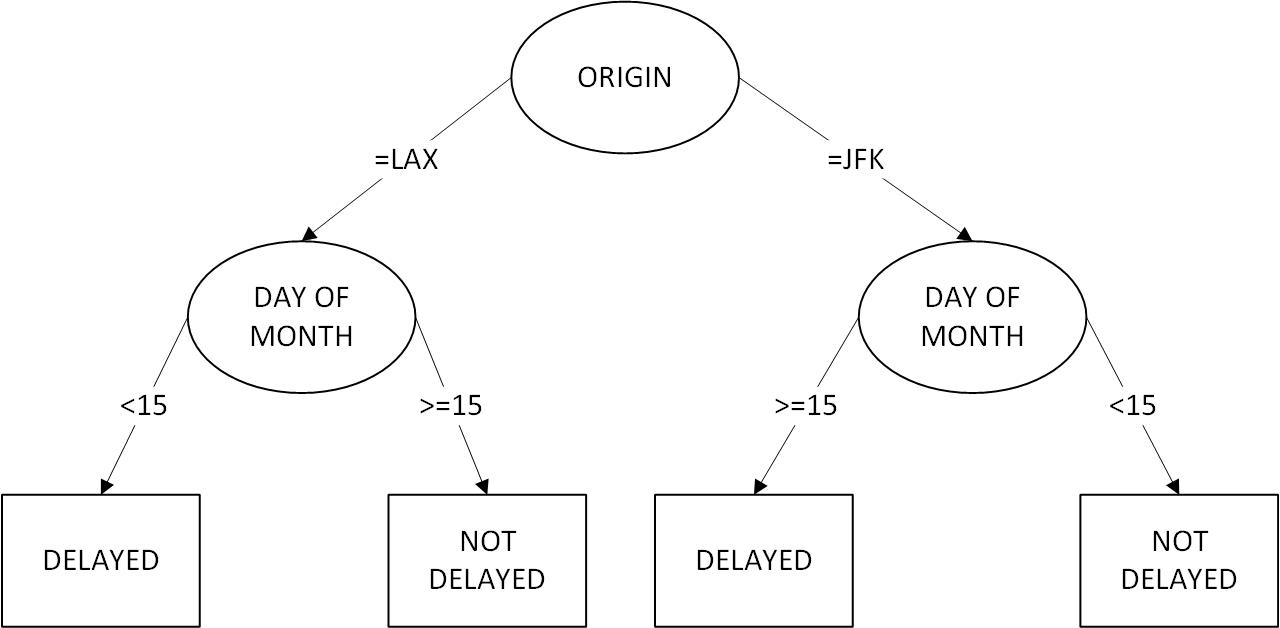
\includegraphics[width=\linewidth]{decisiontree.jpg}
\caption{Sample decision tree for 2 attributes}
\end{figure}

\item{Multiple Linear Regression:}\\
\\---MLM equation---\\
DEPDELAYNEW =\\ 4.2139 *  DAYOFMONTH=26,23,30,12,25,\\
27,24,20,15,28,21,2,14,7,3,18,4,17,10,8 +\\
3.7402 * DAYOFMONTH=15,28,21,2,14,\\
7,3,18,4,17,10,8 +\\
4.9167 * DAYOFMONTH=18,4,17,10,8 +\\
3.503  * DAYOFMONTH=17,10,8 +\\
6.7863 * DAYOFMONTH=8 +\\
7.2751 * CARRIER=MQ,B6,AA,DL,OO,EV,UA +\\
3.4147 * CARRIER=AA,DL,OO,EV,UA +\\
5.0166 * CARRIER=EV,UA +\\
5.03 * ORIGIN=DEN,LAX,JFK,EWR,BOS,ORD +\\
-3.6498 * ORIGIN=EWR,BOS,ORD +\\
5.4878 * ORIGIN=BOS,ORD +\\
9.5943 * DEPTIME=0,2 +\\
26.2807\\
Correlation Coefficient: 0.1919\\\\
---Test Data---\\
Input: 1,2,AA,LAX,1,9,32\\
delay:32.0 predicted delay:41.99\\
Input: 1,2,AA,ORD,2,6,22\\
delay:22.0 predicted delay:53.43\\
Input: 1,2,AA,JFK,2,6,29\\
delay:29.0 predicted delay:51.59\\
\% nearby values: 33.34\%
\end{itemize}

\item{Working code:}
\begin{itemize}
\item{Classifier:}
The classifier class is utilized to build the classification model. The sample code for a J48 classifier in Java to predict class of first instance of the training data is as shown below:-\\
$J48\ j48tree = new\ J48();\\
String\ classes[] = \{ "notdelayed", "delayed" \};\\
DataSource\ data = new\ DataSource("j48train.arff");\\
Instances\ instances = data.getDataSet();\\
int classindex=instances.numAttributes() - 1;\\
instances.setClassIndex(classindex);\\
j48tree.buildClassifier(instances);\\
double \ predictedclass=j48tree.classifyInstance(instances.instance(1));\\
System.out.println(classes[(int)predictedclass]);$



\item{Regressor:}
The regression class is utilized to build the multiple linear regression model. The code for this class in Java to predict delay in flight departure time in minutes is as shown below:-\\
$LinearRegression\ reg = new\ LinearRegression();\\
DataSource\ data = new\ DataSource("regtrain.arff");\\
Instances\ instances = data.getDataSet();\\
int\ classindex=instances.numAttributes() - 1;\\
instances.setClassIndex(classindex);\\
reg.buildClassifier(instances);\\
double\ predicteddelay = reg.classifyInstance(instances.instance(1));\\
System.out.println(predicteddelay);\\
$

\end{itemize}

\item{Demo and sample findings: Here are the observations from running these algorithms on the data:}
\begin{itemize} 
\item{Classifier:}
	For the given data, the J48 algorithm creates a decision tree model with 142 leaf nodes and a total tree size of 208 nodes. It gives an accuracy of 86.39\% on the training data as compared to NBTree which gives 85.80\% accuracy. As for other classification models like Decision Table, Naive Bayes and Random Forest, the accuracy of prediction on test data is less than that of J48 classifier. Thus, we use the J48 decision tree for our classifier model and for the given data attributes, we can say it works pretty well for predicting if a flight will be delayed or not. As for time complexity of classifying a given instance in our data, it will take constant time equal to the height of our decision tree generated. \\
\begin{center}
\begin{tabular}{| l | l | l |}
    \hline
    Algorithm & Model base & Accuracy \\ \hline
    J48 & Tree & 86.39\% \\ \hline
    DecisionTable & Rules & 86.29\% \\ \hline
	NBTree & Tree & 85.80\% \\ \hline
	Naive Bayes & Bayes & 85.75\% \\ \hline
	RandomForest & Forest & 84.41\% \\ \hline
    \end{tabular}
\end{center}
    \ \\Some observations made about the attributes from the j48 decision tree model:-
    \begin{itemize}
    \item{The attribute Departure time is the topmost node in our decision tree. This means that this attribute has the highest effect on delay of a flight, which makes sense as well.   }
    \item{Next, we have the day of month, origin and carrier following with their effect on delay in decreasing order.  }
    \item{Surprisingly, day of week does not have much of an effect on the delay as was previously expected.}
    \end{itemize}
\item{Regressor:}
	The multiple linear regressor model generated from the given data set has a low correlation coefficient. We say the predicted delay is a good enough estimate if it is within 10 minutes of the actual delay in minutes. The given attributes can provide a rough estimate of this delay but in real, there are many more attributes required in order to accurately predict flight departure delay in minutes. Hence, this model is only as good as the attributes present in the data set that can explain the delay in departure time of a flight.\\
    Some observations made about the attributes from the regression model:-
    \begin{itemize}
    \item{The correlation coefficient value of the model is 0.1919 which means there is some relation between the chosen explanatory variables and the response variable delay in flight but the explanatory variables are not sufficient to explain the change in response variable totally.}
    \item{Departure time has a high coefficient in the linear model which means it has a good amount of statistical influence on the delay in flight. This is consistent with our classification model.}
    \item{Other attributes like day of month, carrier and origin airport also have significant value of their coefficients. Again, this is consistent with out classification model.}
	\end{itemize}    
\end{itemize}
\end{itemize}



\subsection{Stage4 -	User Interface. }\label{sec: 4. User Interface.}
%%%%%%%%%%%%%%%%%%%%%%%%%%%%%%%%%%%%%%%%%%%%%%%%%%%%%%%%%%%%%%%%%%%%%%%%%%%%%%%%%%%%%%%%%%%%%%%%%%%%%%%%%%
\textnormal{
The user interface for this system is a simple-to-use desktop application. The system is initiated by clicking on the application icon on the user's machine. This will be followed by the main screen that allows to select the type of user interacting with the system. The following screen will be drawn up respective to the type of user selected in the previous screen.
}
\begin{figure}
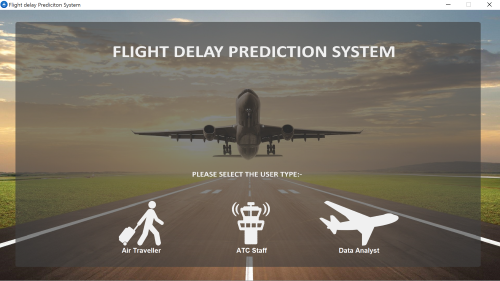
\includegraphics[width=\linewidth]{mainscreen.png}
\caption{Main screen of the application.}
\end{figure}
\begin{itemize} 
\item{User Interface screens and the flow of the application are as below:-}
\begin{itemize} 
\item{Fig. 4. shows the main screen that appears at the start of the application. The three options to the user are to select the user type that can be accessed by mouse click.} 

\item{Fig. 5. shows the input screen for the Air Traveller or the ATC Staff users. Note that the inputs required for both these users are the same. The inputs required here are in the drop down boxes next to their respective labels.}
\end{itemize}
\begin{figure}
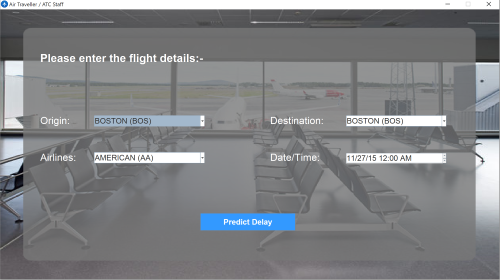
\includegraphics[width=\linewidth]{secondscreen.png}
\caption{User Input screen of the application.}
\end{figure}
\item{Information/Result messages displayed after user interaction are as below:-}
\begin{figure}
\centerline{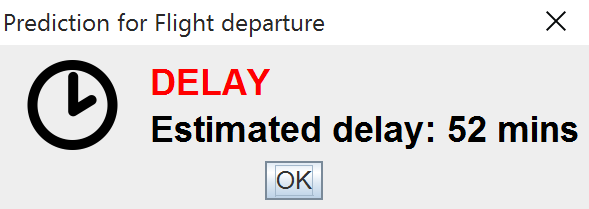
\includegraphics{delay.png}}
\caption{Dialog Box displayed when flight is predicted to be delayed.}
\end{figure}
\begin{figure}
\centerline{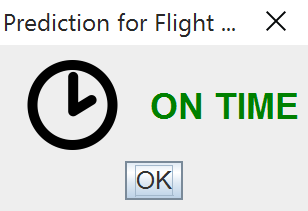
\includegraphics{ontime.png}}
\caption{Dialog Box displayed when flight is predicted to be on time.}
\end{figure}
\begin{itemize}
\item{Fig. 6. and Fig. 7. show the possible outcomes' dialog box when the user presses the predict button in the input screen.}
\end{itemize}
\item{Error messages shown for wrong user inputs are as below:-}
\begin{itemize}
\item{Fig. 8. shows the error message box that appears when the user inputs are such that the origin and the destination of the flights are kept the same.}
\item{The error in the Date/Time field is not shown on the screen but the default value for this field is taken as the input. This is because of the default inbuilt nature of the input field.}

\item{ The error messages in response to data range constraints violations.}
\begin{figure}
\centerline{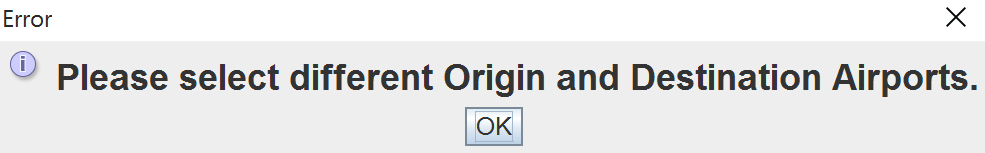
\includegraphics[width=\linewidth]{error.png}}
\caption{Error dialog for wrong user input.}
\end{figure}	
\end{itemize}
\end{itemize}




%\section{Project Highlights.}\label{sec:7. Project Highlights.}
%%%%%%%%%%%%%%%%%%%%%%%%%%%%%%%%%%%%%%%%%%%%%%%%%%%%%%%%%%%%%%%%%%%%%%%%%%%%%%%%%%%%%%%%%%%%%%%%%%%%%%%%%%
%\textnormal{
\begin{itemize} 
\item{}
Only working applications will be acceptable at project completion. A running demo shoul be presented to your project advisor at a date to be specified after the second midterm. A version of your application shall be installed in a machine to be specifed later during the semester. Your final submissiom package will also include a final LaTeX report modeled after this document, as well as a Power Point Presentation.
\item{}
The presentation (7 to 8 minutes) should include at least the following items (The order of the slides is important):
\begin{enumerate}
\item{}
Title: Project Names (authors and affiliations)
\item{}
Project Goal
\item{}
Outline of the presentation
\item{}
Description
\item{}
Pictures are essential. Please include Interface snapshots exemplyfing tthe different modes of users's interaction.
\item{}
Project Stumbling Blocks
\item{}
Data collection, Flow Diagram, Integrity Constraints
\item{}
Sample Findings
\item{}
Future Extensions
\item{}
Acknowledgements
\item{}
References and Resources used(libraries, languages, web resources)
\item{}
Demo(3 minutes)
\end{enumerate}
Please follow the sample presentation mock up that is posted on Sakai.
\item{}
By Dec 1 your group should have completed the final submission. This includes a presentation (7 to 8 minutes) to your project advisor as well as a convincing  demo of your project functionalities (3 minutes): every group member should attend the demo (and presentation) indicating clearly  and specifically his/her contribution to the project.  This wil allow us to evaluate all students in a consistent and fair manner.
\item{}
Thank you, and best of luck!
\end{itemize}
}

\begin{thebibliography}{1}

  \bibitem{kohavi1996scaling} R. Kohavi, 'Scaling Up the Accuracy of Naive-Bayes Classifiers: A Decision-Tree Hybrid',
  CiteSeer, pp. 202--207, 1996.
  
  \bibitem{hall2007decision} M. Hall, 'A decision tree-based attribute weighting filter for naive Bayes',
  Elsevier, vol. 20, no. 2, pp. 120--126, 2007.
  
  \bibitem{michalski2013machine} R. S. Michalski and J. G. Carbonell and T. M. Mitchell, 'Machine learning: An artificial intelligence approach', Springer Science \& Business Media, 2013.

	\bibitem{rish2001empirical} I. Rish, 'IJCAI 2001 workshop on empirical methods in artificial intelligence', IBM New York, 
  vol. 3, no. 22, pp. 41--46, 2001.
  
  \bibitem{mahmood2014analyzingnb} D. Y. Mahmood and M. A. Hussein, 'AnalyzingNB, DT and NBTree IntrusionDetection Algorithms', Journal of Zankoy Sulaimani-Part A (JZS-A), 
  vol. 16, no. 1, pp. 1, 2014.
    
  \bibitem{bl}Transtats.bts.gov, 'RITA | BTS | Transtats', 2015. [Online]. Available: \url{http://www.transtats.bts.gov/DL_SelectFields.asp?Table_ID=236&DB_Short_Name=On-Time}. [Accessed: 01- Nov- 2015].
  
  \end{thebibliography}

%\bibliographystyle{IEEEtran}
%\bibliography{IEEEabrv,mainbib}
%\bibliography{mainbib}

\end{document}